\section{Appendix} \label{sec: Appendix}
The appendix contains code listening and other large information parts that contain partial or complete relevance to the reports topic. 
\subsection{C code Part III} \label{subsec: C code}
\inputencoding{latin1}
\lstinputlisting[style=CStyle,caption={GPIO\_game.c fill contained C code.},label=lst: GPIO_game_c fill contained C code]{../seven_seg_ip/seven_seg_ip.sdk/seven_seg1/src/seven_seg1.c}


\subsection{Errors}\label{subsec: Errors}
\subsubsection{Implementation Error [Place 30-574] Poor placement for routing between an I/O pin and BUFG} \label{subsubsec: Poor placement for routing between an I/O pin and BUFG}
\href{https://wiki.nus.edu.sg/pages/viewpage.action?pageId=167808307}{Poor placement for routing between an I/O pin and BUFG} is a state where a clk signal is routed to anon clock net or a non clock signal is routed to clock net like a posedge or negedge clk signal.
Now it seems this clock placement error that occurs by implementing the project is somewhat related to the decoder. As the decoder module is commented out of the top level block the error is not there any more. Still the source or what pin shall causing the issue could not be located at first.
The issue was that the in the decoder initialization the clk and rst pin where switched.


\subsubsection{Board file}\label{subsubsec: Board fil}q
The following error was generated due to the use of the chip set while generating the Vivado project instead of configure the project with the board file. 
\begin{figure}[H]
	\centering
	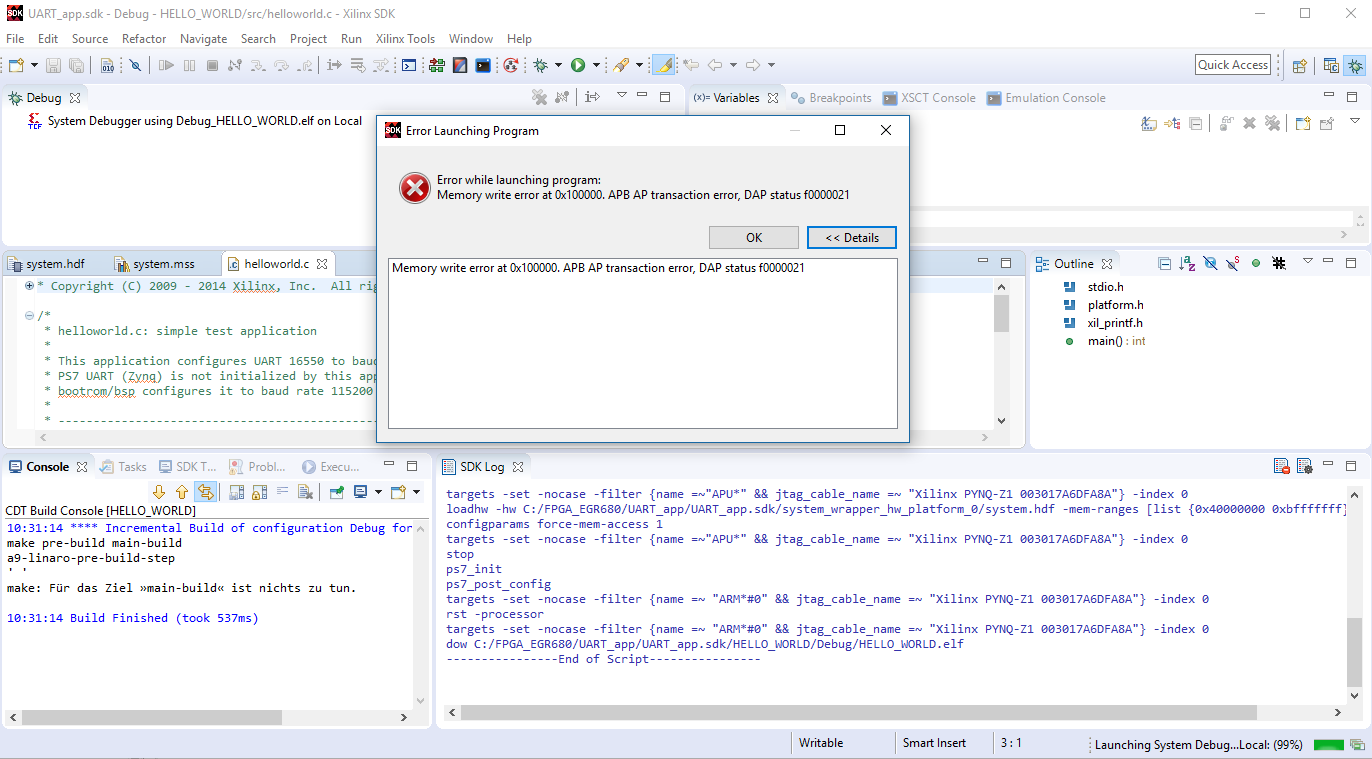
\includegraphics[width=1.0\textwidth]{01_images/Vivado_lab4_part1_SecondErrorSDK.PNG}
	\caption{Error SDK Part I.}
	\label{fig: Vivado_lab4_part1_SecondErrorSDK}
\end{figure}

